% Rendered with pdflatex. NeurIPS-style theme (single column, Times-like serif).
\documentclass[10pt]{article}
\usepackage[letterpaper,left=1.1in,right=1.1in,top=0.8in,bottom=0.8in]{geometry}
\usepackage[T1]{fontenc}
\usepackage{amsmath,amssymb}
\usepackage{newtxtext,newtxmath}   % Times-like serif (NeurIPS look)
\usepackage{graphicx}
\usepackage{booktabs}
\usepackage{float}
\usepackage[font=small,labelfont=bf,skip=4pt]{caption}
\usepackage{subcaption}
\usepackage{titlesec}
\titleformat{\section}{\large\bfseries}{\thesection}{0.6em}{}
\titleformat{\subsection}{\normalsize\bfseries}{\thesubsection}{0.6em}{}
\titlespacing*{\section}{0pt}{6pt}{2pt}
\setlength{\parskip}{1pt}
\usepackage[colorlinks=true,allcolors=blue]{hyperref}

\newcommand{\abc}{$\alpha,\beta$-CROWN}
\newcommand{\linf}{$\ell_\infty$}
\newcommand{\eps}{$\varepsilon$}

\begin{document}

\begin{center}
  {\LARGE\bfseries Bound-Propagation Robustness Verification of an\\[2pt]
   MNIST Classifier: $\alpha,\beta$-CROWN vs.\ Marabou}\\[10pt]
  {\normalsize Jaemin Paek}\\[2pt]
  \rule{\textwidth}{0.4pt}
\end{center}

\begin{center}\textbf{Abstract}\end{center}
\begin{quote}\small
We verify the local \linf{} robustness of a small fully-connected MNIST classifier with
\abc{} and compare it, on identical instances, with the SMT-based verifier Marabou used in
a previous study. The two tools agree on every shared verdict and on per-sample robustness
thresholds, which we use as a soundness cross-check. The interesting differences are
quantitative: the speed gap is not constant but opens up at a specific \eps{}, the
verification effort shifts from cheap bounds to branch-and-bound within a narrow \eps{} band,
all counterexamples are found by the attack rather than by search, and the choice of
branching heuristic --- not the solver itself --- decides success on hard instances.
\end{quote}

\section{Setup}
\textbf{Model and data.} The network is a fully-connected classifier $784\!\to\!64\!\to\!32
\!\to\!10$ with ReLU activations (96 hidden units), exported to ONNX and reused unchanged
from the Marabou study so that both tools verify \emph{the same} network on \emph{the same}
inputs. Inputs are MNIST test images, normalized with mean $0.1307$ and std $0.3081$ (pixel
values lie in $[-0.4242, 2.8215]$).

\textbf{Property.} For an input $x$ with true label $L$ and radius \eps{}, we verify local
\linf{} robustness: for all $x'$ with $\lVert x'-x\rVert_\infty \le \varepsilon$ (clipped to
the valid range), the network keeps $L$ as the arg-max. We encode this per instance as
VNNLIB, with the perturbation applied in the \emph{normalized} input space to match the
Marabou queries exactly; UNSAT $\Rightarrow$ verified, SAT $\Rightarrow$ falsified. \abc{}
runs on CPU with branch-and-bound (no Gurobi) and the \texttt{kfsb} branching heuristic.

\section{Results and Interpretation}
\textbf{Phase 1 --- scan (100 samples, $\varepsilon=0.05$).} 96 verified robust, 4 falsified
(samples 8, 33, 92, 96), 0 timeouts; mean $0.21$\,s/instance.

\textbf{Phase 2 --- thresholds.} The smallest falsified \eps{} is $0.03$ for sample 8 and
$0.05$ for sample 33; sample 0 stays robust through $\varepsilon=0.20$. These match the
Marabou thresholds exactly.

\textbf{The speed advantage is \eps{}-dependent, not constant.} On the robust sample 0, the
two tools are essentially tied at small radii ($\varepsilon=0.01$: Marabou $0.39$\,s, \abc{}
$0.30$\,s) and remain comparable up to $\varepsilon=0.11$ (Marabou $1.0$\,s). Marabou then
degrades sharply --- $6.2$\,s at $\varepsilon=0.12$ and its $300$\,s timeout at
$\varepsilon\ge0.19$ --- while \abc{} rises only to $1.5$\,s at $\varepsilon=0.20$
(Fig.~\ref{fig:runtime}). The often-quoted ${\sim}270\times$ gap is therefore a property of
the \emph{tail}; the honest summary is ``matched until $\varepsilon\approx0.11$, after which
SMT search falls off a cliff.''

\textbf{Where the effort goes, and a sharp transition.} Decomposing how each of the 100
instances is settled (Fig.~\ref{fig:breakdown}) shows that cheap incomplete CROWN bounds
suffice for all 100 at $\varepsilon\le0.02$, but only 5 at $\varepsilon=0.20$; the
branch-and-bound share rises steeply in a narrow band around $\varepsilon\approx0.12$--$0.15$.
The verification difficulty is concentrated, not spread evenly across \eps{}.

\textbf{All counterexamples come from the attack, never from search.} Across every \eps{},
falsified instances are resolved by the PGD attack (\texttt{unsafe-pgd}) and never by
branch-and-bound (\texttt{unsafe-bab} $=0$). For this network the cheap attack is already
strong enough to falsify; the expensive complete search is spent almost entirely on
\emph{proving} robustness. Recovered counterexamples are clear misclassifications (e.g.,
sample 8: $5\!\to\!6$; 33: $4\!\to\!0$; 92: $9\!\to\!4$; 96: $1\!\to\!9$), each a small
perturbation inside the \eps{}-ball (Fig.~\ref{fig:cex}).

\begin{figure}[H]
  \centering
  \begin{subfigure}{0.49\textwidth}\centering
    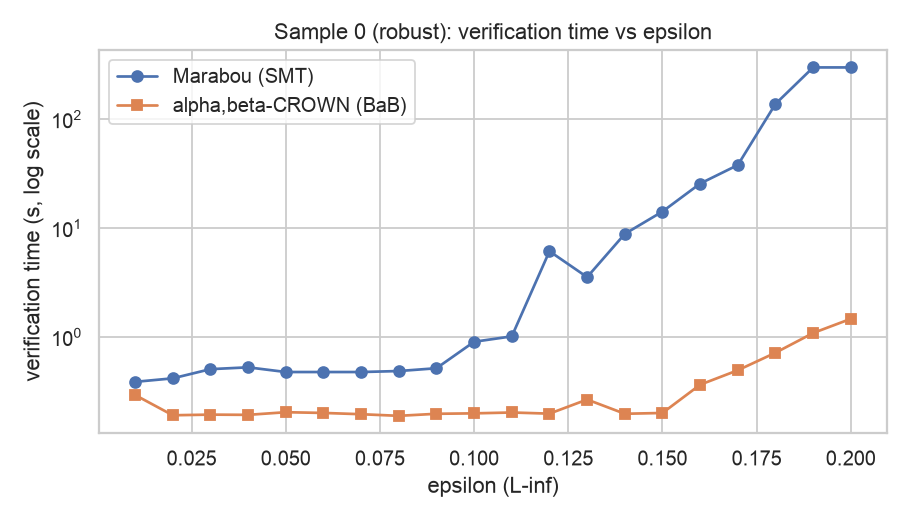
\includegraphics[width=\textwidth]{results/fig_runtime_vs_eps.png}
    \caption{}\label{fig:runtime}
  \end{subfigure}\hfill
  \begin{subfigure}{0.49\textwidth}\centering
    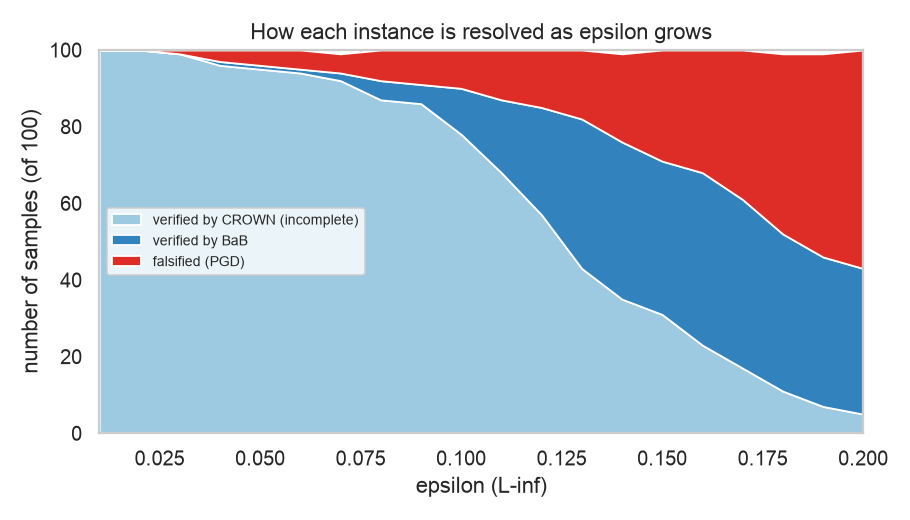
\includegraphics[width=\textwidth]{results/fig_breakdown_area.png}
    \caption{}\label{fig:breakdown}
  \end{subfigure}
  \caption{(a) Verification time vs.\ \eps{} for robust sample 0 (log scale): comparable
  until $\varepsilon\approx0.11$, then Marabou times out while \abc{} stays near $1.5$\,s.
  (b) How the 100 instances are resolved as \eps{} grows; the branch-and-bound share rises
  sharply around $\varepsilon\approx0.12$--$0.15$.}
  \label{fig:plots}
\end{figure}

\begin{figure}[H]
  \centering
  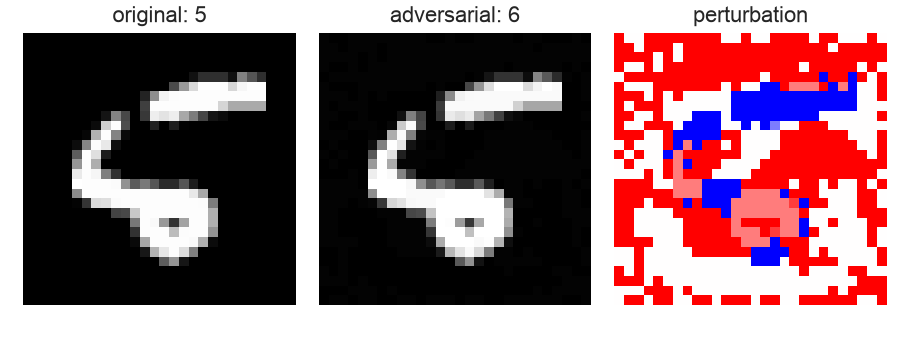
\includegraphics[width=0.46\textwidth]{results/cex_s8.png}
  \caption{Counterexample for sample 8 at $\varepsilon=0.05$ (original $\mid$ adversarial
  $\mid$ perturbation): an \linf{} perturbation flips the prediction $5\!\to\!6$.}
  \label{fig:cex}
\end{figure}

\section{Comparison with Marabou}
\begin{table}[H]
  \centering\small
  \begin{tabular}{lll}
    \toprule
     & \abc{} & Marabou \\
    \midrule
    Method & linear relaxation + branch-and-bound & SMT (Reluplex) \\
    Interface & declarative YAML + VNNLIB & imperative Python API \\
    Verdicts on shared instances & identical & identical \\
    Robust sample, $\varepsilon=0.20$ & ${\sim}1.5$\,s & $300$\,s (timeout) \\
    Single small query (cold start) & ${\sim}2.5$\,s & ${\sim}0.5$\,s \\
    \bottomrule
  \end{tabular}
\end{table}

Beyond the table, three points are worth making from the experiments. First, the
\emph{agreement} itself is a result: matching the property across tools required applying
\eps{} in the normalized space inside the VNNLIB, and the identical thresholds ($0.03$,
$0.05$) confirm both that the encoding is correct and that the two independent engines are
mutually consistent. Second, ``ease of use'' cut both ways: \abc{}'s config-driven batch mode
made a 100-sample sweep a single run, but reaching a working setup required handling
tool-specific friction (a mandatory \texttt{gurobipy} import even when Gurobi is unused, and a
CPU-only build), whereas Marabou's Python API is more direct for a one-off query. Third, the
recovered \emph{counterexamples need not match}: Marabou's non-strict violation encoding
($\text{output}[j]\ge\text{output}[L]$) can return a point whose arg-max ties the true class,
while \abc{}'s PGD returns a strict misclassification --- both are valid witnesses of the same
non-robustness.

\section{Strengths and Limitations}
\textbf{Strengths.} \abc{} scales gracefully where SMT does not: it certified all 100 test
samples cheaply (enabling a full robustness-radius distribution --- 43/100 remain robust
beyond $\varepsilon=0.20$), and it resolved the large-\eps{} robust cases that drove Marabou
to timeout.

\textbf{Limitations observed.} (i) It is \emph{not} universally faster: a single small query
costs ${\sim}2.5$\,s cold versus Marabou's ${\sim}0.5$\,s, because per-process start-up
dominates for tiny models; the advantage appears only once start-up is amortized over a batch.
(ii) Success can hinge on the branching heuristic rather than the solver: on the hardest
instance (sample 22, $\varepsilon=0.2$), \texttt{kfsb} verified in $31$\,s, \texttt{fsb} timed
out, and the \texttt{babsr} heuristic crashed with an upstream \texttt{AttributeError}. The
default \texttt{kfsb} worked, but the configuration surface is large and not uniformly robust.

\end{document}
